
% this file is called up by thesis.tex
% content in this file will be fed into the main document

%: ----------------------- introduction file header -----------------------
\chapter{Results and conclusions}

\graphicspath{{results/figures/}}

% ----------------------------------------------------------------------
%: ----------------------- introduction content ----------------------- 
% ----------------------------------------------------------------------

\section{Performance}

% table with machine configurations

Performance test were performed on two machines which configuration is presented in table~\ref{tab:test_configuration}. PhysX scene with one emitter was used. Results were rendered in two resolutions - 640~x~480 and 1280~x~960

%Present graphs with frame rate depending on number of particle simulated. Note that decrease in performance comes also from simulation cost, not only from rendering.

%Show second set of graphs showing time to render one frame depending on number of particles. 

%Show table showing how resolution affects performance of algorithms when number of particles is kept constant.

%Show table showing speedup of isosurface algorithm.

\begin{table}   
    \caption[Configuration of test machines]{\textbf{Configuration of test machines} - Machine 1 is a high performance gaming desktop, machine 2 is a middle class multimedia laptop.}
    \centering
    \begin{tabular}{ l | p{4.5cm} | p{4.5cm} }
                                         & machine 1                                             & machine 2 \\ \hline
        CPU                           & Intel Core i7 2600k 3.4 GHz, 4 cores  & Inte Core i7 2630M 2.0 GHz, 4 cores \\ \hline
        GPU                           & Nvidia GeForce GTX 560 Titanium        &  Nvidia GeForce GT 540M \\ \hline
        Physical memory       & 8 GB                                                      & 6GB \\
    \end{tabular}
    \label{tab:test_configuration}
\end{table}

%\figuremacro{curvature_640_480}{Performance of screen space rendering with curvature flow at 640x480}{Some description}
%\figuremacro{curvature_1280_960}{Performance of screen space rendering with curvature flow at 1280x960}{Some description}
\figuremacro{bilateral}{Performance of screen space rendering with bilateral Gaussian smoothing}{Some description}
\figuremacro{curvature_100it}{Performance of screen space rendering curvature flow smoothing}{100 iterations were performed for each frame.}
\figuremacro{isosurface_3th}{Performance of isosurface extraction}{3 threads were used}

Figures \ref{bilateral}, \ref{curvature_100it} and \ref{isosurface_3th} presents graphs of frames per second on the number of simulated particles. Maximum frame rate was restrained to 60. Those three graphs takes both simulation and rendering time into consideration. First thing to notice is that screen space techniques are much more vulnerable to increasing resolution than isosurface extraction. This is due to much more complex shader programs used, especially in curvature flow smoothing. 

Isosurface extraction (figure~\ref{isosurface_3th} runs on CPU and is it much more dependent on number of particles rendered than on resolution. Rendering is smooth for less than 10000 particles. 

\begin{table}
   \caption[Performance comparison]{\textbf{Performance comparison} of all rendering algorithms. Screen space methods were run with 60000 particles, isosurface extraction was run using 3 threads.}
   \centering
   \begin{tabular} { l | r | c | r }
      Algorithm                                       &            resolution              &          machine           &          Frame (ms)      \\ \hline \hline
      Bilateral Gaussian smoothing        &           640x480                &              1                  &           10.0                    \\ \hline
      Bilateral Gaussian smoothing        &           1280x960              &              1                  &           13.8                    \\ \hline
      Bilateral Gaussian smoothing        &           640x480                &              2                  &           51.9                    \\ \hline
      Bilateral Gaussian smoothing        &           1280x960              &              2                  &           63.5                    \\ \hline \hline

      Curvature flow smoothing 100 it. &           640x480                &              1                  &           15.6                    \\ \hline
      Curvature flow smoothing 100 it. &          1280x960               &              1                  &           27.8                    \\ \hline
      Curvature flow smoothing 100 it. &           640x480                &              2                  &           73.1                    \\ \hline
      Curvature flow smoothing 100 it. &          1280x960               &              2                  &           134.1                  \\ \hline \hline

      Curvature flow smoothing 60 it.   &           640x480                &              1                  &           13.7                \\ \hline
      Curvature flow smoothing 60 it.   &          1280x960               &              1                  &           22.0                \\ \hline
      Curvature flow smoothing 60 it.   &           640x480                &              2                  &           65.7                    \\ \hline
      Curvature flow smoothing 60 it.   &          1280x960               &              2                  &           104.5               \\ \hline \hline

      Isosurface extraction                    &          640x480                &              1                  &            160.4               \\ \hline     
      Isosurface extraction                    &          1280x960               &              1                  &           161.5                   \\ \hline      
      Isosurface extraction                    &          640x480                &              2                  &            302.1               \\ \hline
      Isosurface extraction                    &          1280x960               &              2                  &           312.3               \\ 
   \end{tabular}
   \label{tab:frame_time}
\end{table}

\figuremacro{perf_comp_machine1}{Performance comparison of algorithms}{Time to render one frame (excluding simulation time) on number of particles. Tests were run on machine 1 in 1280 x 960, isosurface extraction was run using 3 threads, curvature flow smoothing performed 100 iterations.}

Figure~\ref{perf_comp_machine1} presents graph of time to render single frame (in milliseconds, excluding simulation time) on number of particles for all three algorithms implemented. It can be seen that all of them have linear complexity, however isosurface extraction has much higher constant. Curvature flow takes around 15 milliseconds more than bilateral Gaussian smoothing, regardless of number of particles simulated. 

In table~\ref{tab:frame_time} times for rendering one frame for different algorithms, resolutions and machines are gathered. They were measured for 60000 particles. It confirms statement that isosurface extraction is not suitable for rendering large number of particles. Only screen space techniques are fast enough, although on lower performance machines curvature flow is also to expensive.

\figuremacro{isosurface_speedup}{Speedup of multithreaded version of isosurface extraction}{Tests performed on machine 1 for 60000 particles. Only rendering and surface extraction time were taken into account.} 

Figure~\ref{isosurface_speedup} shows graph of isosurface extraction algorithm speedup. Entire domain was divided into 4x4x4 = 64 cubes. The performance stops growing after 3 threads. This is due to the fact that CPU has only 4 cores and PhysX simulation was performed simultaneously on one of them. What is more cube division was quite coarse and around half of 64 blocks were empty. On the other side decreasing cube size would lead to increased overhead due to cubes overlaping. 

\subsection{Visual appearance}

Figure~\ref{fig:visual_appearance} shows comparison of visual appearance of waterfall scene rendered with different algorithms. Screen space algorithms include reflection, refraction based on fluid depth and color based on fluid depth. Isosurface extraction does not use depth based refraction and fluid color. Best quality is offered by curvature smoothing with 100 iterations. Bilateral Gaussian smoothing yields similar results as curvature flow with 60 iterations. Fluid rendered using surface extraction is also realistic and it doesn't have artifacts on edges like screen space methods. It's advantage is that it produces surface which can be rendered by game's engine using existing materials. Screen space methods requires custom shaders which can be harder to integrate with game engine. 

\begin{figure}[ht]
\begin{minipage}[b]{0.5\linewidth}
\centering
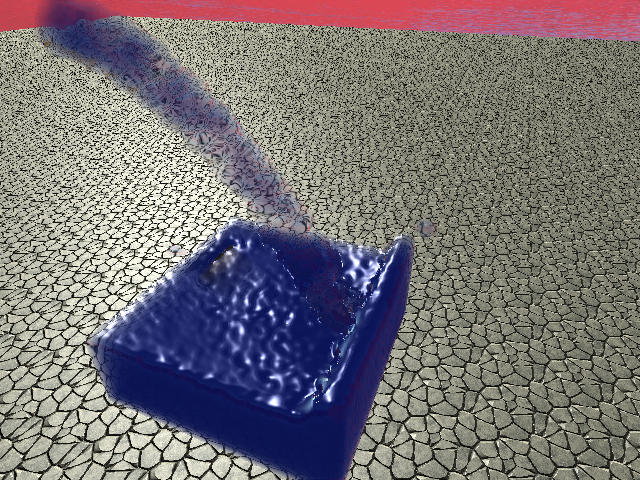
\includegraphics[width=1\textwidth]{bilateral_gauss}
(a) Bilateral Gaussian
\end{minipage}
\hspace{0.5cm}
\vspace{0.5cm}
\begin{minipage}[b]{0.5\linewidth}
\centering
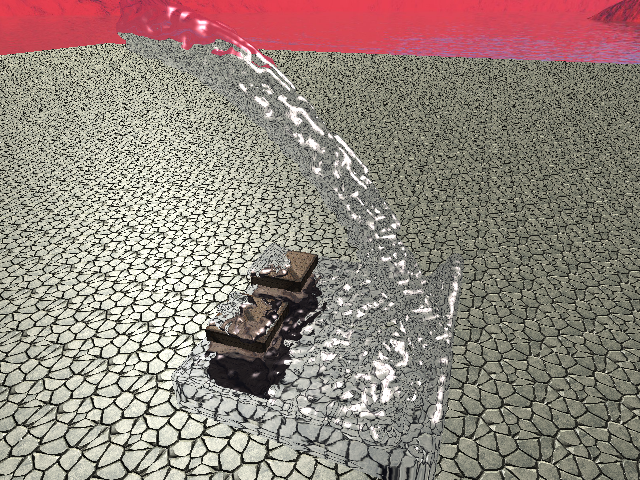
\includegraphics[width=1\textwidth]{isosurface}
(b) Isosurface extraction
\end{minipage}
\vspace{0.5cm}
\begin{minipage}[b]{0.5\linewidth}
\centering
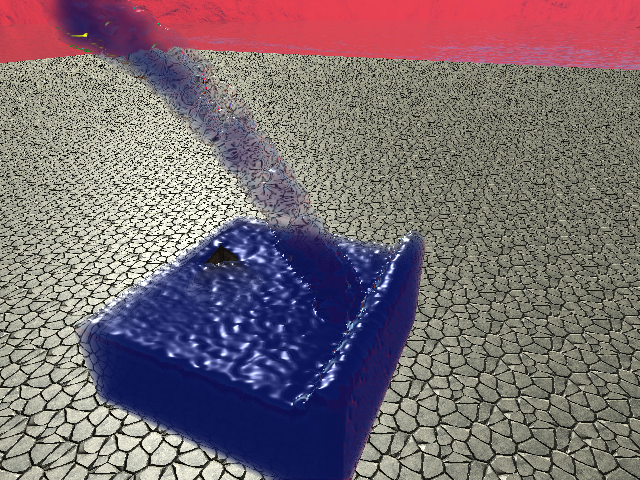
\includegraphics[width=1\textwidth]{curvature_flow_60}
(c) Curvature flow, 60 iterations
\end{minipage}
\hspace{0.5cm}
\begin{minipage}[b]{0.5\linewidth}
\centering
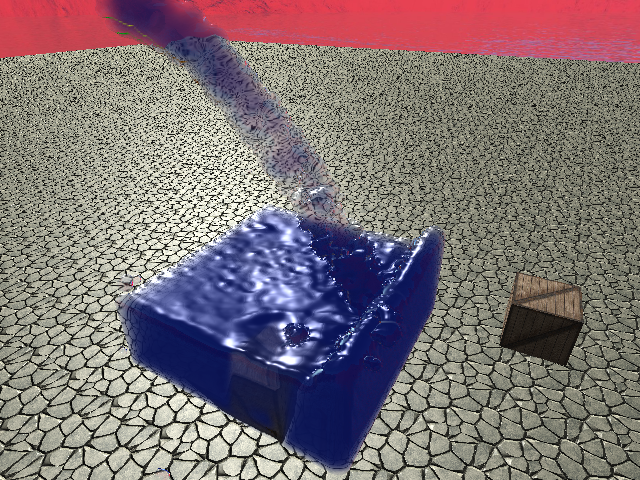
\includegraphics[width=1\textwidth]{curvature_flow_100}
(d) Curvature flow 100 iterations
\end{minipage}
\caption{Comparison of visual appearance of different algorithms.}
\label{fig:visual_appearance}
\end{figure}

\subsection{Conclusions}
I have presented 3 algorithms for rendering particle fluid. All of them can be used in real time simulations in computer games. However each of them has different application. Isosurface extraction is good for rendering small amount of particles - less than 10000. It can be used to render small fountains, water flowing from a tap or blood. To speedup isosurface extraction it can be implemented on GPU. 
When higher number of particles are simulated screen space techniques can be used. Bilateral Gaussian smoothing can be used on lower performance and curvature flow smoothing on higher performance hardware. 


% ----------------------------------------------------------------------



